\section{Materiais e Métodos}
\subsection{Materiais}
Para captar e realizar a leitura do ruído elétrico foram utilizados um microcontrolador e um pedaço de estanho.
\subsubsection{Arduino UNO}
O Arduino Uno (Fig 1) é uma placa de microcontrolador baseado no ATmega328 (datasheet). Ele tem 14 pinos de entrada/saída digital (dos quais 6 podem ser usados como saídas PWM), 6 entradas analógicas, um cristal oscilador de 16MHz, uma conexão USB, uma entrada de alimentação uma conexão ICSP e um botão de reset. Ele contém todos os componentes necessários para suportar o microcontrolador, simplesmente conecte a um computador pela porta USB ou alimentar com uma fonte ou com uma bateria e tudo pronto para começar.

O Arduino foi responsável pela leitura do ruído elétrico em uma de suas portas analógicas e a partir disso fazer o processamento dessa leitura a fim de gerar um número aleatório.

\begin{figure}[H]
	\label{fig1}
	\begin{centering}
		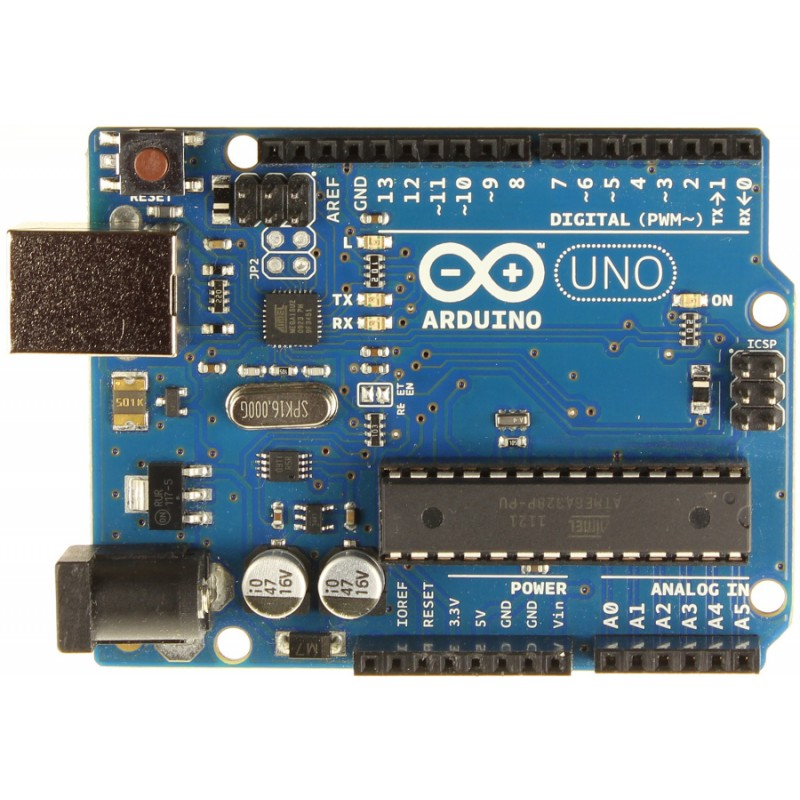
\includegraphics[width = 400pt]{img/arduino.jpg}
		\caption{Arduino UNO}
	\end{centering}	
		
\end{figure}

\subsubsection{Estanho}

Foi utilizado um pedaço de estanho na porta do microcontrolador como aparato para amplificar a captação de interferência eletromagnética. De forma que facilitasse a leitura dos dados pelo microcontrolador.
 \begin{figure}[H]
 	\label{fig2}
 	\begin{centering}
 		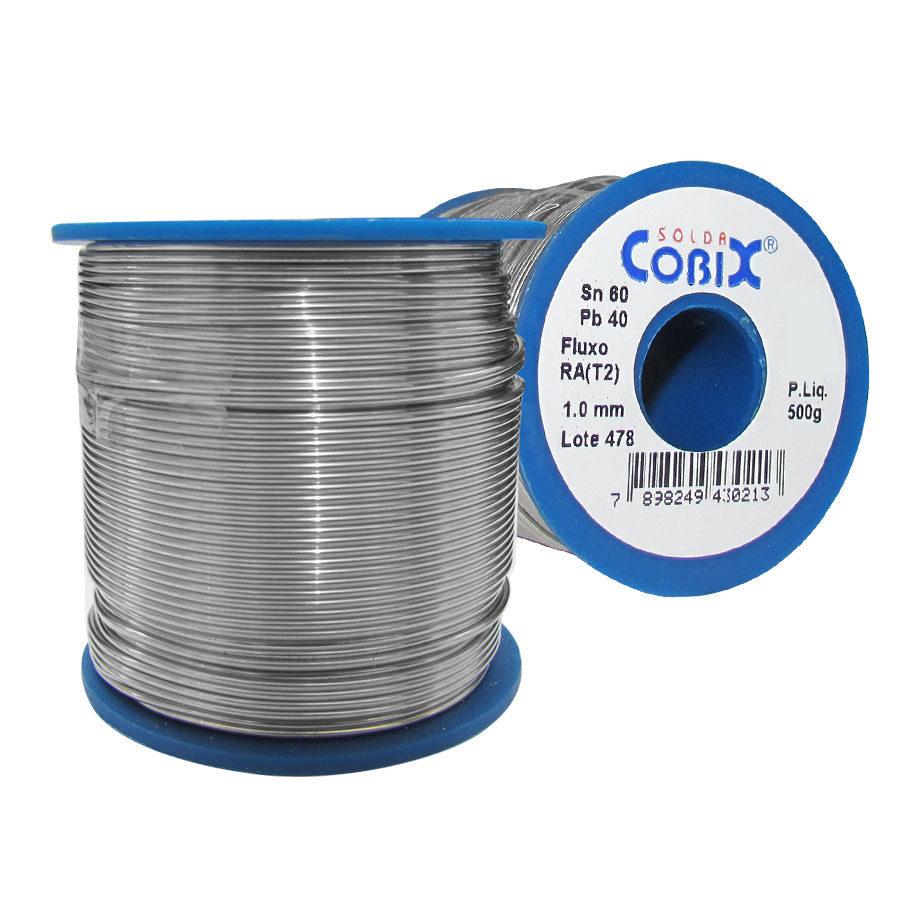
\includegraphics[width = 200pt]{img/estanho.jpg}
 		\caption{Estanho}
 	\end{centering}	
 		
 \end{figure}

\subsection{Métodos}